\documentclass{beamer}

% \usepackage{beamerthemesplit} // Activate for custom appearance

\title{Building Artificial Life and Multi-Agent simulations using the Breve engine}
\author{Wouter Bulten, Frank Dorssers \& Robert-Jan Drenth}
\date{\textit{ACAIS: Life}, June 6th 2013}

\usebackgroundtemplate{%
  \vbox to 1.8\paperheight{\vfil\hbox to 1.66\paperwidth{\hfil
\includegraphics[height=0.4in]{ACAIS2013_logodatum}\hfil}\vfil}

}
\definecolor{acaisred}{rgb}{0.75,0.19,0.1}

\setbeamercolor{title}{fg=acaisred}
\setbeamercolor{frametitle}{fg=acaisred}
\setbeamercolor{structure}{fg=acaisred}

\begin{document}

\frame{
\titlepage}

\frame{
	\center{
		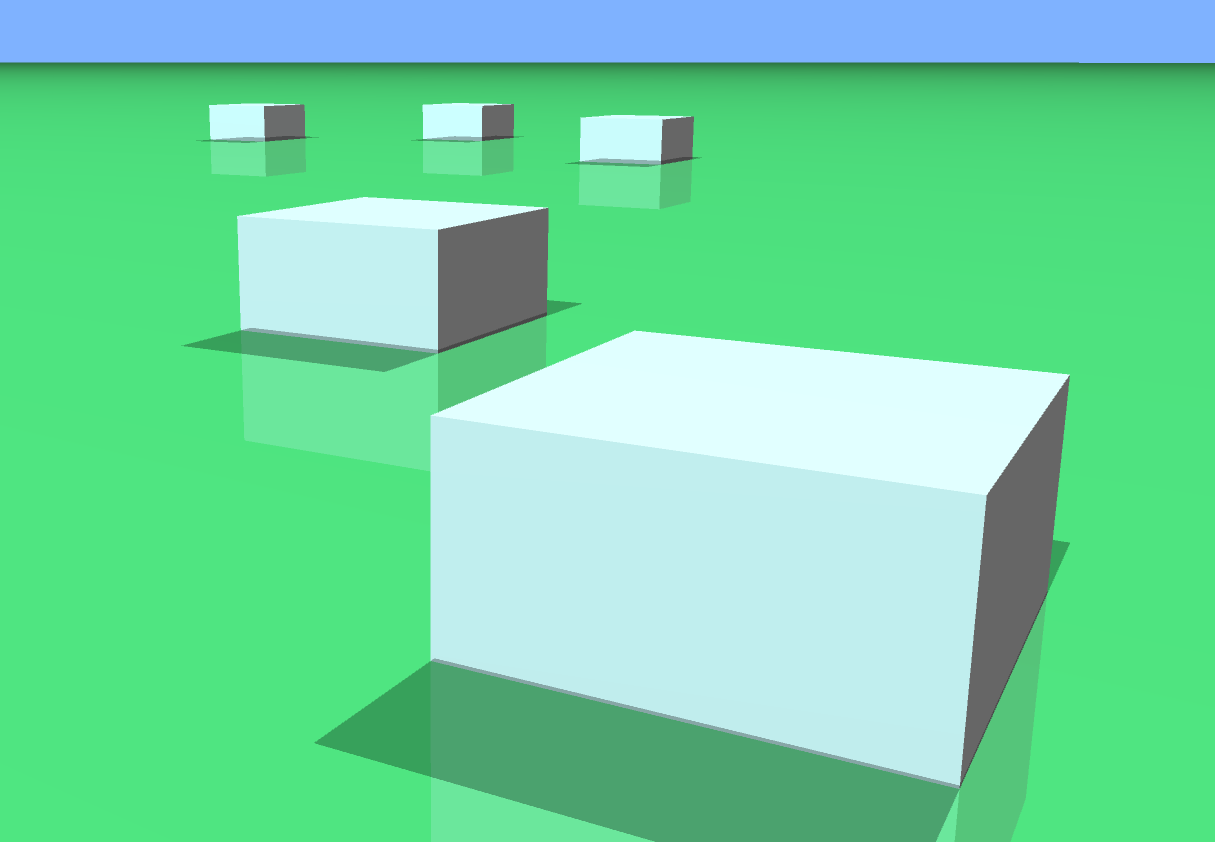
\includegraphics[width=\textwidth]{agents.png}
	}
}
\section[Outline]{}
\frame{
\frametitle{Overview}
\tableofcontents}

\section{Introduction by examples}

\frame{
	\frametitle{The evolution of leadership}
}

\section{What is Breve?}
\frame{

}

\section{Basis of a simulation}
\frame{

}

\section{Building a simulation}
\frame{

}

\section{Adding complexity}
\frame{

}

\end{document}
